
\documentclass[letterpaper,hide notes,xcolor={table,svgnames},pdftex,10pt]{beamer}
\def\showexamples{t}


%\usepackage[svgnames]{xcolor}

%% Demo talk
%\documentclass[letterpaper,notes=show]{beamer}

\usecolortheme{crane}
\setbeamertemplate{navigation symbols}{}

\usetheme{MyPittsburgh}
%\usetheme{Frankfurt}

%\usepackage{tipa}

\usepackage{hyperref}
\usepackage{graphicx,xspace}
\usepackage[normalem]{ulem}
\usepackage{multicol}
\usepackage{amsmath,amssymb,amsthm,graphicx,xspace}
\newcommand\SF[1]{$\bigstar$\footnote{SF: #1}}

\usepackage[default]{sourcesanspro}
\usepackage[T1]{fontenc}

\newcounter{tmpnumSlide}
\newcounter{tmpnumNote}

% old question code
%\newcommand\question[1]{{$\bigstar$ \small \onlySlide{2}{#1}}}
% \newcommand\nquestion[1]{\ifdefined \presentationonly \textcircled{?} \fi \note{\par{\Large \textbf{?}} #1}}
% \newcommand\nanswer[1]{\note{\par{\Large \textbf{A}} #1}}


 \newcommand\mnote[1]{%
   \addtocounter{tmpnumSlide}{1}
   \ifdefined\showcues {~\tiny\fbox{\arabic{tmpnumSlide}}}\fi
   \note{\setlength{\parskip}{1ex}\addtocounter{tmpnumNote}{1}\textbf{\Large \arabic{tmpnumNote}:} {#1\par}}}

\newcommand\mmnote[1]{\note{\setlength{\parskip}{1ex}#1\par}}

%\newcommand\mnote[2][]{\ifdefined\handoutwithnotes {~\tiny\fbox{#1}}\fi
% \note{\setlength{\parskip}{1ex}\textbf{\Large #1:} #2\par}}

%\newcommand\mnote[2][]{{\tiny\fbox{#1}} \note{\setlength{\parskip}{1ex}\textbf{\Large #1:} #2\par}}

\newcommand\mquestion[2]{{~\color{red}\fbox{?}}\note{\setlength{\parskip}{1ex}\par{\Large \textbf{?}} #1} \note{\setlength{\parskip}{1ex}\par{\Large \textbf{A}} #2\par}\ifdefined \presentationonly \pause \fi}

\newcommand\blackboard[1]{%
\ifdefined   \showblackboard
  {#1}
  \else {\begin{center} \fbox{\colorbox{blue!30}{%
         \begin{minipage}{.95\linewidth}%
           \hspace{\stretch{1}} Some space intentionally left blank; done at the blackboard.%
         \end{minipage}}}\end{center}}%
         \fi%
}



%\newcommand\q{\tikz \node[thick,color=black,shape=circle]{?};}
%\newcommand\q{\ifdefined \presentationonly \textcircled{?} \fi}

\usepackage{listings}
\lstset{%
  keywordstyle=\bfseries,
  aboveskip=15pt,
  belowskip=15pt,
  captionpos=b,
  identifierstyle=\ttfamily,
  escapeinside={(*@}{@*)},
  stringstyle=\ttfamiliy,
  frame=lines,
  numbers=left, basicstyle=\scriptsize, numberstyle=\tiny, stepnumber=0, numbersep=2pt}

\usepackage{siunitx}
\newcommand\sius[1]{\num[group-separator = {,}]{#1}\si{\micro\second}}
\newcommand\sims[1]{\num[group-separator = {,}]{#1}\si{\milli\second}}
\newcommand\sins[1]{\num[group-separator = {,}]{#1}\si{\nano\second}}
\sisetup{group-separator = {,}, group-digits = true}

%% -------------------- tikz --------------------
\usepackage{tikz}
\usetikzlibrary{positioning}
\usetikzlibrary{arrows,backgrounds,automata,decorations.shapes,decorations.pathmorphing,decorations.markings,decorations.text}

\tikzstyle{place}=[circle,draw=blue!50,fill=blue!20,thick, inner sep=0pt,minimum size=6mm]
\tikzstyle{transition}=[rectangle,draw=black!50,fill=black!20,thick, inner sep=0pt,minimum size=4mm]

\tikzstyle{block}=[rectangle,draw=black, thick, inner sep=5pt]
\tikzstyle{bullet}=[circle,draw=black, fill=black, thin, inner sep=2pt]

\tikzstyle{pre}=[<-,shorten <=1pt,>=stealth',semithick]
\tikzstyle{post}=[->,shorten >=1pt,>=stealth',semithick]
\tikzstyle{bi}=[<->,shorten >=1pt,shorten <=1pt, >=stealth',semithick]

\tikzstyle{mut}=[-,>=stealth',semithick]

\tikzstyle{treereset}=[dashed,->, shorten >=1pt,>=stealth',thin]

\usepackage{ifmtarg}
\usepackage{xifthen}
\makeatletter
% new counter to now which frame it is within the sequence
\newcounter{multiframecounter}
% initialize buffer for previously used frame title
\gdef\lastframetitle{\textit{undefined}}
% new environment for a multi-frame
\newenvironment{multiframe}[1][]{%
\ifthenelse{\isempty{#1}}{%
% if no frame title was set via optional parameter,
% only increase sequence counter by 1
\addtocounter{multiframecounter}{1}%
}{%
% new frame title has been provided, thus
% reset sequence counter to 1 and buffer frame title for later use
\setcounter{multiframecounter}{1}%
\gdef\lastframetitle{#1}%
}%
% start conventional frame environment and
% automatically set frame title followed by sequence counter
\begin{frame}%
\frametitle{\lastframetitle~{\normalfont(\arabic{multiframecounter})}}%
}{%
\end{frame}%
}
\makeatother

\makeatletter
\newdimen\tu@tmpa%
\newdimen\ydiffl%
\newdimen\xdiffl%
\newcommand\ydiff[2]{%
    \coordinate (tmpnamea) at (#1);%
    \coordinate (tmpnameb) at (#2);%
    \pgfextracty{\tu@tmpa}{\pgfpointanchor{tmpnamea}{center}}%
    \pgfextracty{\ydiffl}{\pgfpointanchor{tmpnameb}{center}}%
    \advance\ydiffl by -\tu@tmpa%
}
\newcommand\xdiff[2]{%
    \coordinate (tmpnamea) at (#1);%
    \coordinate (tmpnameb) at (#2);%
    \pgfextractx{\tu@tmpa}{\pgfpointanchor{tmpnamea}{center}}%
    \pgfextractx{\xdiffl}{\pgfpointanchor{tmpnameb}{center}}%
    \advance\xdiffl by -\tu@tmpa%
}
\makeatother
\newcommand{\copyrightbox}[3][r]{%
\begin{tikzpicture}%
\node[inner sep=0pt,minimum size=2em](ciimage){#2};
\usefont{OT1}{phv}{n}{n}\fontsize{4}{4}\selectfont
\ydiff{ciimage.south}{ciimage.north}
\xdiff{ciimage.west}{ciimage.east}
\ifthenelse{\equal{#1}{r}}{%
\node[inner sep=0pt,right=1ex of ciimage.south east,anchor=north west,rotate=90]%
{\raggedleft\color{black!50}\parbox{\the\ydiffl}{\raggedright{}#3}};%
}{%
\ifthenelse{\equal{#1}{l}}{%
\node[inner sep=0pt,right=1ex of ciimage.south west,anchor=south west,rotate=90]%
{\raggedleft\color{black!50}\parbox{\the\ydiffl}{\raggedright{}#3}};%
}{%
\node[inner sep=0pt,below=1ex of ciimage.south west,anchor=north west]%
{\raggedleft\color{black!50}\parbox{\the\xdiffl}{\raggedright{}#3}};%
}
}
\end{tikzpicture}
}


%% --------------------

%\usepackage[excludeor]{everyhook}
%\PushPreHook{par}{\setbox0=\lastbox\llap{MUH}}\box0}

%\vspace*{\stretch{1}

%\setbox0=\lastbox \llap{\textbullet\enskip}\box0}

\setlength{\parskip}{\fill}

\newcommand\noskips{\setlength{\parskip}{1ex}}
\newcommand\doskips{\setlength{\parskip}{\fill}}

\newcommand\xx{\par\vspace*{\stretch{1}}\par}
\newcommand\xxs{\par\vspace*{2ex}\par}
\newcommand\tuple[1]{\langle #1 \rangle}
\newcommand\code[1]{{\sf \footnotesize #1}}
\newcommand\ex[1]{\uline{Example:} \ifdefined \presentationonly \pause \fi
  \ifdefined\showexamples#1\xspace\else{\uline{\hspace*{2cm}}}\fi}

\newcommand\ceil[1]{\lceil #1 \rceil}


\AtBeginSection[]
{
   \begin{frame}
       \frametitle{Outline}
       \tableofcontents[currentsection]
   \end{frame}
}



\pgfdeclarelayer{edgelayer}
\pgfdeclarelayer{nodelayer}
\pgfsetlayers{edgelayer,nodelayer,main}

\tikzstyle{none}=[inner sep=0pt]
\tikzstyle{rn}=[circle,fill=Red,draw=Black,line width=0.8 pt]
\tikzstyle{gn}=[circle,fill=Lime,draw=Black,line width=0.8 pt]
\tikzstyle{yn}=[circle,fill=Yellow,draw=Black,line width=0.8 pt]
\tikzstyle{empty}=[circle,fill=White,draw=Black]
\tikzstyle{bw} = [rectangle, draw, fill=blue!20, 
    text width=4em, text centered, rounded corners, minimum height=2em]
    
    \newcommand{\CcNote}[1]{% longname
	This work is licensed under the \textit{Creative Commons #1 3.0 License}.%
}
\newcommand{\CcImageBy}[1]{%
	\includegraphics[scale=#1]{creative_commons/cc_by_30.pdf}%
}
\newcommand{\CcImageSa}[1]{%
	\includegraphics[scale=#1]{creative_commons/cc_sa_30.pdf}%
}
\newcommand{\CcImageNc}[1]{%
	\includegraphics[scale=#1]{creative_commons/cc_nc_30.pdf}%
}
\newcommand{\CcGroupBySa}[2]{% zoom, gap
	\CcImageBy{#1}\hspace*{#2}\CcImageNc{#1}\hspace*{#2}\CcImageSa{#1}%
}
\newcommand{\CcLongnameByNcSa}{Attribution-NonCommercial-ShareAlike}

\newenvironment{changemargin}[1]{% 
  \begin{list}{}{% 
    \setlength{\topsep}{0pt}% 
    \setlength{\leftmargin}{#1}% 
    \setlength{\rightmargin}{1em}
    \setlength{\listparindent}{\parindent}% 
    \setlength{\itemindent}{\parindent}% 
    \setlength{\parsep}{\parskip}% 
  }% 
  \item[]}{\end{list}} 




\title{Lecture 25 --- Deadlock, Lock Granularity}

\author{Jeff Zarnett \\ \small \texttt{jzarnett@uwaterloo.ca}}
\institute{Department of Electrical and Computer Engineering \\
  University of Waterloo}
\date{\today}


\begin{document}

\begin{frame}
  \titlepage

 \end{frame}

\begin{frame}
\frametitle{Deadlock}

You should recall from learning about concurrency what deadlock is about, and therefore a brief review only is in order. 

Those in need of a refresher are advised to take a look through previous courses' material to get caught up. 

Others may find this to be review material, but it does deviate in some significant ways from the discussion of deadlocked processes.

\end{frame}

\begin{frame}
\frametitle{Deadlock}
We have already introduced the subject of deadlock and gave an informal definition as all transactions being ``stuck'' (unable to proceed). 

A more formal definition: ``the \textit{permanent} blocking of a set of transactions that either compete for system resources or communicate with each other''. 

There is emphasis on permanent. 

It may be possible for all transactions to be stuck temporarily, because one is waiting for some event (e.g., a read from disk).

\end{frame}

\begin{frame}
\frametitle{Conditions for Deadlock}
Remember, there are four condition necessary for a deadlock to take place:

\begin{enumerate}
	\item \textbf{Mutual Exclusion}
	\item \textbf{Hold-and-Wait}
	\item \textbf{No Preemption}
	\item \textbf{Circular-Wait}
\end{enumerate}

\end{frame}

\begin{frame}
\frametitle{Don't Handle It}

We could choose not to handle deadlock. 

This option is certainly convenient for database system designers! 

While it is tempting and easy to just define a problem as being nothing we need to deal with, that's unrealistic in reality. 

If two transactions get deadlocked, the user may simply see no progress and just feel bad about it. 

\end{frame}

\begin{frame}
\frametitle{Deadlock Prevention}

The first three conditions for deadlock (mutual exclusion, hold and wait, and no preemption) are all necessary for deadlock to be possible. 

If we eliminate one of these three pillars, deadlock is not possible and it is prevented from happening. 

If we prevent the circular wait from occurring, we are still in a world where deadlock can occur. 

We cleverly avoid it taking place based on how we allow locks to occur.

\end{frame}

\begin{frame}
\frametitle{Mutual Exclusion}

This pillar cannot, generally speaking, be disallowed. 

The purpose of  mutual exclusion is to prevent errors like inconsistent state or crashes. 

Getting rid of mutual exclusion to rule out the possibility of deadlock is a cure that is worse than the disease. 

It is therefore not acceptable as a solution.


\end{frame}

\begin{frame}
\frametitle{Hold and Wait}
To prevent the hold-and-wait condition, we must guarantee that when a transaction requests a resource, it does not have any other resource. 

One plausible solution is that the transaction must request all resources at the beginning of the program. 

So if the transaction is going to need resources $R_{1}$, $R_{2}$, and $R_{3}$ at some point in the program: 

All three must be requested right at the beginning and held throughout the transaction.

 No further resources may be requested at any time during execution

\end{frame}


\begin{frame}
\frametitle{No Preemption}
f we violate this condition, it means that we do have preemption: forcible removal of resources from a transaction. 

In the database context, if we have to preempt a transaction, it means the transaction in question is rolled back and then restarted. 

To work out an ordering, transactions are assigned a timestamp. 

If a transaction is rolled back, its timestamp remains the same
\end{frame}


\begin{frame}
\frametitle{Or, Preemption}
There are two approaches for what happens if we need to do pre-emption:

The first is called \alert{wait-die}. 

If a transaction $T_{i}$ requests an item held by $T_{j}$, then the timestamps of these two transactions are compared. 

$T_{i}$ will be allowed to wait if it is older (i.e. its timestamp is a smaller number) than $T_{j}$, otherwise it ``dies'' (is rolled back). 


\end{frame}

\begin{frame}
\frametitle{Or, Preemption}

The second is \alert{wound-wait}. 

If a transaction $T_{i}$ requests an item held by $T_{j}$, then the timestamps of these two transactions are compared. 

If $T_{i}$ is the younger transaction (its timestamp is larger), then $T_{i}$ can wait. 

Otherwise, $T_{j}$ is ``wounded'' by $T_{i}$ and $T_{j}$ is rolled back.

\end{frame}

\begin{frame}
\frametitle{Roll Back}

So, in case of a conflict, one of the two transactions is going to be rolled back. 

And it is always the younger one. 

In either approach there may be unnecessary rollbacks...

\end{frame}

\begin{frame}
\frametitle{Timeout}

Instead we could also have locks that have timeouts. 

When a lock is requested there is a defined maximum time the transaction is willing to wait. 

If that time limit is reached, the transaction rolls back automatically and begins again. 

The obvious difficulty lies in choosing the length of time that the transactions will wait.

\end{frame}

\begin{frame}
\frametitle{Circular Wait}

We have already discussed the idea of using two phase locking to put an ordering on the locks and we need not repeat that yet again. 


\end{frame}

\begin{frame}
\frametitle{Deadlock Detection}

A quick review of the graph algorithm follows, then. 

If resources have only a single instance, we may reduce the graph to a simplified version called the \alert{wait-for} graph. 

This removes the resource boxes from the diagram and indicates that a process $P_{i}$ is waiting for process $P_{j}$ rather than for a resource $R_{k}$ that is held by $P_{j}$. 

An edge $P_{i} \rightarrow P_{j}$ exists in the wait-for graph if and only if the resource allocation graph has a request $P_{i} \rightarrow R_{k}$ and an assignment edge $R_{k} \rightarrow P_{j}$. 

\end{frame}


\begin{frame}
\frametitle{Deadlock Detection}

\begin{center}
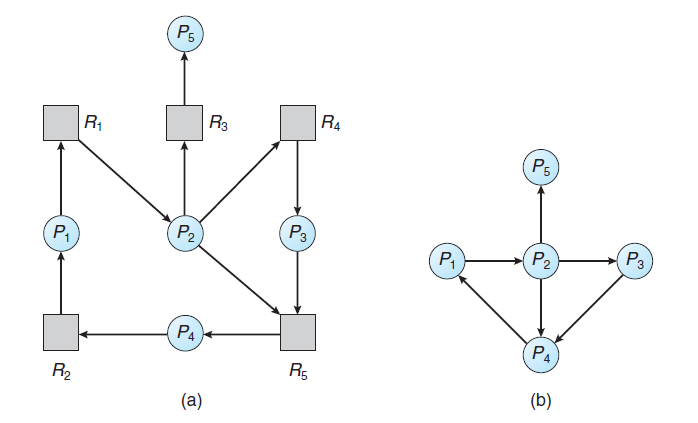
\includegraphics[width=0.75\textwidth]{images/rag-waitfor.png}
\end{center}


\end{frame}


\begin{frame}
\frametitle{Database Deadlock Detection}

Because locks are unique then there is no need to use the resource allocation graph and we can always use the simplified wait-for graph for transactions:

\begin{center}
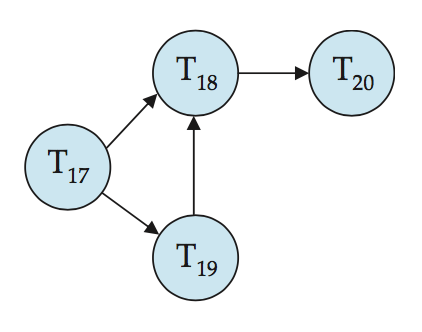
\includegraphics[width=0.45\textwidth]{images/transaction-waitfor.png}
\end{center}


\end{frame}

\begin{frame}
\frametitle{Deadlock Detection is Expensive}

Cycle detection algorithms tend to have runtime characteristics of $\Theta(n^{2})$ where $n$ is the number of nodes in the graph.

How often should the deadlock detection algorithm be run?


\end{frame}

\begin{frame}
\frametitle{Deadlock Recovery}

On the subject of what transaction to select as a victim we already identified the timestamp as one possible way to decide. Or: 

\begin{enumerate}
\item How long the transaction has been executing.
	\item How long is remaining in execution (see the estimates from the execution plan).
	\item What resources the transaction has used.
	\item Future resource requests, if known.
	\item How many times, if any, the transaction has been selected as a victim (to prevent starvation).
\end{enumerate}

\end{frame}


\begin{frame}
\frametitle{Push the Ball Uphill}

We chose a victim, now simply roll that transaction back! 

That would be a total rollback: undo all the steps of the transaction and start from the beginning once again. 

There exists, however, the ability to do a \alert{partial rollback}. 

\end{frame}

\begin{frame}
\frametitle{Partial Rollback}

The goal of the partial rollback is to rollback the transaction back only as much as is necessary to break the deadlock.  

This is accomplished by maintaining the sequence of lock requests and grants.

 By finding the lock(s) that are implicated in the deadlock, we can roll back a transaction to where it obtained the first of such locks.

\end{frame}



\begin{frame}
\frametitle{Lock Granularity}

Locks' extents constitute their \alert{granularity}: that is, how much data is being protected by such a lock.

\alert{Coarse-grained} locking is easier to implement, but it can significantly reduce opportunities for parallelism. 

\alert{Fine-grained locking} requires more careful design, increases locking overhead and is more prone to bugs (deadlock etc).

 
\end{frame}

\begin{frame}
\frametitle{Granularity Hierarchy}
In the database we could define multiple levels of granularity. 

\begin{center}
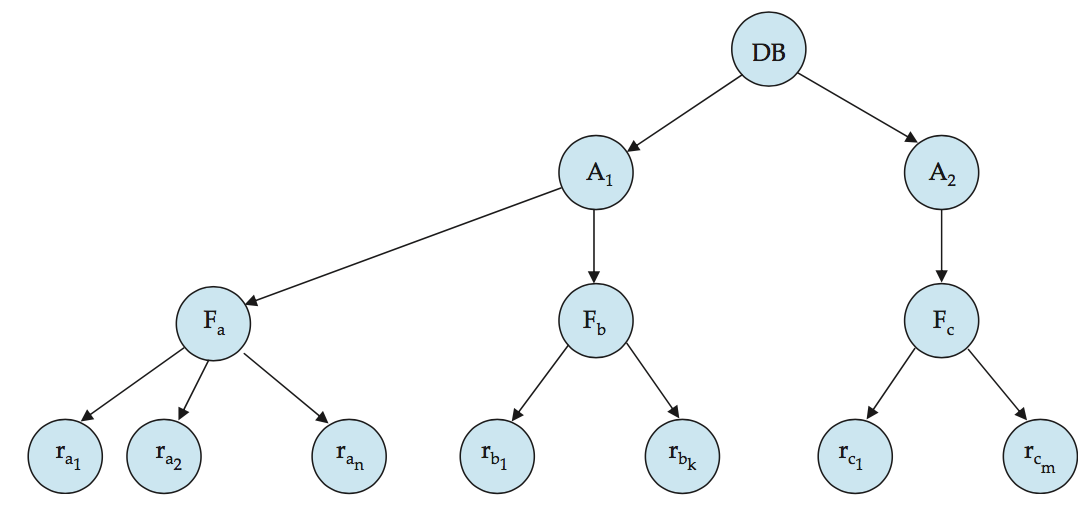
\includegraphics[width=0.7\textwidth]{images/granularity-hierarchy}
\end{center}


\end{frame}

\begin{frame}
\frametitle{Intention Lock Modes}

A more efficient route is \alert{intention lock modes}, which are put on the ancestors of a node before the node is locked.

These intention locks can be checked while traversing the tree. The following modes are possible:

\begin{itemize}
	\item \textbf{Shared} (S)
	\item \textbf{Exclusive} (X) 
	\item \textbf{Intention Shared} (IS) 
	\item \textbf{Intention Exclusive} (IX) 
	\item \textbf{Shared Intention Exclusive} (SIX)
\end{itemize} 


\end{frame}

\begin{frame}
\frametitle{Intention Lock Rules}

Then a transaction must follow the six rules below:

\begin{enumerate}
	\item All attempts to lock must observe the table (below) as to whether they are permitted to proceed (or wait).
	\item The transaction must lock the root of the tree first (in any mode, but it must pick one).
	\item A node $n$ can be locked in \textbf{S} or \textbf{IS} mode only if the parent of $n$ is locked in either \textbf{IX} or \textbf{IS} mode.
	\item A node $n$ can be locked in \textbf{X}, \textbf{SIX}, or \textbf{IX} mode only if the parent of $n$ is locked in either \textbf{IX} or \textbf{SIX} mode.
	\item A node $n$ may only be locked if the transaction has not previously unlocked any nodes.
	\item A node $n$ may only be unlocked if none of the children of $n$ are locked by this transaction.
\end{enumerate}

Locks must be acquired in a top-down manner and then released in a bottom-up manner. 

\end{frame}

\begin{frame}
\frametitle{Lock Compatibility Matrix}

\begin{center}
\begin{tabular}{|c|c|c|c|c|c|} \hline
	Compatibility & \textbf{IS} & \textbf{IX} &\textbf{S} &\textbf{SIX} &\textbf{X}\\ \hline
\textbf{IS} & \checkmark &\checkmark  & \checkmark & \checkmark & $\times$ \\ \hline
\textbf{IX} & \checkmark & \checkmark & $\times$ & $\times$ & $\times$	\\ \hline
\textbf{S} & \checkmark & $\times$ & \checkmark & $\times$ & $\times$ \\ \hline
\textbf{SIX} & \checkmark & $\times$ & $\times$ & $\times$ & $\times$ \\ \hline
\textbf{X} & $\times$ & $\times$ & $\times$ & $\times$ & $\times$ \\ \hline
	
\end{tabular}
\end{center}

\end{frame}














\end{document}

